\documentclass[11pt]{article}

\usepackage[utf8]{inputenc}
\usepackage[T1]{fontenc}
\usepackage{lmodern}
\usepackage[spanish]{babel}
\usepackage[margin=2.5cm]{geometry}
\usepackage{graphicx}
\usepackage{booktabs}
\usepackage{hyperref}
\usepackage{amsmath}
\usepackage{caption}

\title{Golden Hour: Acceso Vial a Salud Resolutiva en Perú \\
\large Un Análisis Geoespacial de Lambayeque, Cusco y Loreto}
\author{Luis Felipe Abriojo Vargas \\ Ciencia de Datos, 2026-II}
\date{\today}

\begin{document}
\maketitle

\begin{abstract}
Este reporte cuantifica, mediante ruteo sobre la red vial real (OSMnx +
NetworkX, sin motor comercial ni Docker), el tiempo de acceso por carretera
a un establecimiento de salud con capacidad resolutiva (categoría II-1 en
adelante) para la población de tres departamentos peruanos -- Lambayeque
(costa), Cusco (andino) y Loreto (amazónico) -- y compara ese acceso entre
perfiles de auto, bicicleta y a pie. En Lambayeque, el 84.8\% de la
población accede en auto en 30 minutos o menos a una instalación
resolutiva, pero con una desigualdad marcada (Gini de acceso ponderado por
población = 0.659): el acceso rural promedia 24.1 minutos frente a 7.9 en
zonas urbanas, y el distrito peor ubicado (Cañaris, Ferreñafe) promedia más
de 180 minutos ponderados. El desvío entre distancia en línea recta y
distancia real de ruteo es de 1.17x en mediana para Lambayeque (terreno
plano), una cifra que se espera crezca sustancialmente en Cusco y Loreto
por relieve y desconexión vial, respectivamente. El 36.6\% de los registros
nacionales de RENIPRESS carecen de coordenadas válidas, una limitación
central del análisis discutida en detalle.
\end{abstract}

\tableofcontents

\section{Introducción y planteamiento del problema}

En emergencias obstétricas o traumatológicas graves, la ``hora dorada'' es
la ventana en la que el paciente debe llegar a un establecimiento con
capacidad de resolver la emergencia (cirugía, cesárea). En el sistema
peruano, un puesto de salud (categoría I-1) puede estabilizar pero no
resolver: solo los establecimientos de categoría II-1 en adelante tienen
capacidad quirúrgica. La pregunta que este proyecto busca responder es
concreta: \emph{¿cuánto tarda realmente, por carretera, la población de una
región dada en llegar a un establecimiento con esa capacidad, y dónde están
las peores brechas?}

La palabra difícil es ``realmente''. Una línea recta en un mapa no es una
carretera. Un establecimiento que figura en el registro puede estar
cerrado. Una coordenada del registro puede estar en el hemisferio
equivocado. Gran parte del valor de este análisis -- y de su defensa --
está en el tratamiento explícito de esos problemas, no en el número final.

El alcance se limita a tres departamentos, uno por macrorregión geográfica
(costa, sierra, selva), precisamente para poder contrastar: una región
costera y una amazónica no deberían comportarse igual ante el mismo
problema de acceso, y ese contraste es el punto analítico central del
ejercicio.

\section{Fuentes de datos}

\begin{itemize}
  \item \textbf{Oferta (RENIPRESS/SUSALUD)}: registro nacional de
  establecimientos de salud, descargado el 2026-09-04 desde
  \url{datosabiertos.gob.pe} (snapshot de agosto 2026, 36{,}004 registros
  nacionales). Licencia Open Data Commons Attribution. El portal está
  detrás de un WAF que bloquea el User-Agent por defecto de
  \texttt{requests}/\texttt{curl} (HTTP 418); se requiere un User-Agent de
  navegador.
  \item \textbf{Demanda (MINEDU/SIGMED)}: capa nacional única de ``Centros
  Poblados'' (153{,}400 puntos), descargada el 2026-09-04 desde el botón de
  descarga de \url{sigmed.minedu.gob.pe/descargas/} (sin URL pública
  documentada; se identificó inspeccionando la red del navegador). La
  página anuncia actualización al 05/02/2020, pero el \texttt{Last-Modified}
  real del servidor es 2021-12-10. No incluye población por punto.
  \item \textbf{Red vial (OpenStreetMap)}: extracto de Perú de Geofabrik
  (\url{download.geofabrik.de/south-america/peru-latest.osm.pbf},
  256\,MB, descargado el 2026-09-04), documentado como fuente pero no usado
  como input directo del grafo -- ver Metodología, motor de ruteo.
  \item \textbf{Límites administrativos}: INEI no publica un enlace de
  descarga directa estable para polígonos distritales; se usó el GeoJSON
  derivado republicado en \url{github.com/juaneladio/peru-geojson} (1834
  distritos, 8 con geometría nula -- ninguno en los 3 departamentos de
  alcance).
  \item \textbf{Población distrital (INEI, Censo 2017)}: sin dataset
  descargable en \texttt{datosabiertos.gob.pe} (su endpoint CKAN
  \texttt{package\_search} no está habilitado), se extrajo del PDF
  ``Tomo I'' de cada departamento (\url{inei.gob.pe}, Cuadro N.º 1,
  población censada por provincia y distrito), verificando que la suma de
  distritos coincide exactamente con el total impreso de provincia y
  departamento en las 3 fuentes.
\end{itemize}

\section{Metodología}

\subsection{Definición de capacidad resolutiva}

Un establecimiento es resolutivo si y solo si su estado operativo es
\texttt{ACTIVO} y su categoría normalizada es II-1, II-2, II-E, III-1,
III-2 o III-E. El campo \texttt{CATEGORIA} de RENIPRESS no es una cadena
limpia: el 30.65\% de los 3{,}631 registros en los 3 departamentos de
alcance llevan el valor literal \texttt{"0"} en vez de una categoría real
(23.75\% a nivel nacional), y se normalizan a \texttt{SIN\_CATEGORIA} --
tratado como no resolutivo, nunca como capacidad asumida. La normalización
usa una expresión regular tolerante a variantes de formato
(\texttt{src/validation.py:normalize\_category}), no solo un mapeo de los
valores observados hoy.

\subsection{Reglas de validación}

Implementadas en \texttt{src/validation.py} y ejecutadas sobre los
3{,}631 establecimientos y 21{,}095 centros poblados de los 3
departamentos:

\begin{itemize}
  \item \textbf{Coordenadas nulas o cero}: 32.36\% de RENIPRESS (0\% en
  SIGMED). Se conservan en el registro pero se excluyen del cómputo
  geoespacial.
  \item \textbf{Fuera del bbox de Perú}: 0 casos en ambas fuentes.
  \item \textbf{Lat/lon invertidos}: 0 casos detectados; la corrección
  automática solo se aplica cuando el intercambio mueve el punto
  \emph{dentro} del bbox de Perú, nunca a ciegas.
  \item \textbf{Punto fuera de su distrito declarado}: 13.1\% de RENIPRESS
  y 1.7\% de SIGMED (con coordenadas válidas) caen fuera del polígono de
  su propio \texttt{UBIGEO}, con tolerancia de 500\,m. Se conserva el
  registro con una advertencia -- no se puede saber si el error está en el
  ubigeo o en la coordenada sin revisión manual.
  \item \textbf{Códigos duplicados}: 0 casos en ambas fuentes.
  \item \textbf{Codificación}: el archivo de RENIPRESS es UTF-8 con BOM y
  delimitado por \texttt{;} (no por coma, pese a la extensión \texttt{.csv}).
\end{itemize}

\subsection{Motor de ruteo y parámetros}

Se usó \textbf{OSMnx + NetworkX}, sin OSRM/Docker: la máquina de desarrollo
no tiene Docker Desktop ni WSL2 instalados, y levantarlos exige reinicio
del sistema y permisos de administrador -- el mismo tipo de cambio pesado
que se evitó al descartar \texttt{pyrosm} (requiere compilador de C++ no
disponible). Los grafos se descargan en vivo vía
\texttt{osmnx.graph\_from\_polygon()} contra Overpass API, con caché en
disco. La instancia por defecto (\texttt{overpass-api.de}) estuvo
inalcanzable durante más de una hora en la sesión de cómputo; el pipeline
reintenta con backoff y hace \emph{failover} a espejos públicos
(\texttt{overpass.kumi.systems}, \texttt{overpass.osm.ch}) -- documentado
como hallazgo legítimo sobre la fragilidad de la infraestructura abierta,
no como error del pipeline.

Velocidades: auto usa la imputación por tipo de vía de OSMnx (con
respaldo de 40\,km/h); bicicleta y a pie usan velocidades constantes de
12 y 4.5\,km/h respectivamente (\texttt{config.md}).

La matriz completa origen\,$\times$\,instalación (auto) se calcula con
\emph{un} Dijkstra de fuente única por instalación -- no un cálculo por
par --, ya que el número de instalaciones (14--27 resolutivas por
departamento) es muchísimo menor que el de puntos de demanda; esto da la
matriz completa esencialmente gratis. La matriz también enruta a los
candidatos I-3/I-4 (no solo a los ya-resolutivos), precisamente para que
el simulador de escenarios de la Fase 4 pueda recalcular cobertura al
``elevar'' un candidato sin volver a rutear en vivo.

Con 21{,}095 puntos de demanda en los 3 departamentos, por encima del
tope de 5{,}000 fijado en \texttt{config.md}, se aplicó un muestreo
estratificado por departamento y ponderado por población (no por conteo
de puntos): cada departamento recibe una cuota proporcional a su
población total estimada, y dentro de cada departamento el muestreo
pondera cada centro poblado por una estimación de población derivada del
censo distrital (ver más abajo).

\subsection{Estimación de población por punto de demanda}

SIGMED no trae población por centro poblado. Se usa la jerarquía real del
campo \texttt{CAPITAL} de SIGMED (verificada en los datos: 0 = no capital,
3 = capital distrital, 2 = capital provincial, 1 = capital departamental
-- 25 casos a nivel nacional, exactamente los 24 departamentos + Callao)
para repartir la población censal 2017 de cada distrito entre sus centros
poblados, asignando más masa poblacional a las capitales. Es un supuesto
documentado, no una medición -- ver Limitaciones.

\subsection{Definición de métricas}

Todas las métricas (\texttt{src/metrics.py}) son funciones puras que
reciben y devuelven \texttt{DataFrame}, ponderadas por población salvo
que se indique lo contrario:

\begin{itemize}
  \item \textbf{Tiempo de acceso} $t_{\min}(i)$: minutos en auto desde el
  punto $i$ a la instalación resolutiva más cercana.
  \item \textbf{Bandas de cobertura}: \% de población en $\leq$30,
  30--60, 60--120 y $>$120 minutos, más una banda de ``sin ruta''.
  \item \textbf{Acceso ponderado por población}, agregado por distrito,
  provincia y departamento.
  \item \textbf{Ranking de brechas críticas}: distritos peor ubicados por
  acceso ponderado.
  \item \textbf{Coeficiente de Gini} de acceso, vía el área bajo la curva
  de Lorenz -- se eligió sobre una medida de varianza simple por estar
  acotado en [0,1], ser estándar en la literatura de acceso a salud, y ser
  comparable entre departamentos de tamaño y tiempo medio muy distintos.
  \item \textbf{Contraste urbano/rural}: un punto es urbano si su
  población estimada supera 2{,}000 habitantes o si es alguna capital
  (\texttt{config.md}).
  \item \textbf{Cruce con ruralidad distrital}: de las dimensiones
  sugeridas por el enunciado (pobreza, ruralidad, población bajo 5,
  altitud), se usó ruralidad por ser la única calculable directamente de
  los datos ya en mano, sin adquirir una fuente adicional.
\end{itemize}

\section{Resultados}

\subsection{Cobertura y desigualdad de acceso (Lambayeque)}

\begin{table}[h]
\centering
\caption{Cobertura poblacional por banda de tiempo de acceso (auto, instalación resolutiva más cercana)}
\label{tab:coverage-bands}
\resizebox{\textwidth}{!}{\begin{tabular}{lrr}
\toprule
Banda de acceso & Población & \% de población \\
\midrule
0-30 min & 1822077.98 & 78.39 \\
30-60 min & 238262.30 & 10.25 \\
60-120 min & 100957.89 & 4.34 \\
>120 min & 26075.45 & 1.12 \\
unroutable & 557.52 & 0.02 \\
\bottomrule
\end{tabular}}
\end{table}

\begin{table}
\caption{Tiempo de acceso ponderado por población, por departamento}
\label{tab:access-by-department}
\begin{tabular}{lrrrr}
\toprule
department & population_weighted_mean_t_min & total_population & n_demand_points & pct_population_unroutable \\
\midrule
LAMBAYEQUE & 17.77 & 1135934.65 & 1834.00 & 0.05 \\
\bottomrule
\end{tabular}
\end{table}


\begin{figure}[h]
\centering
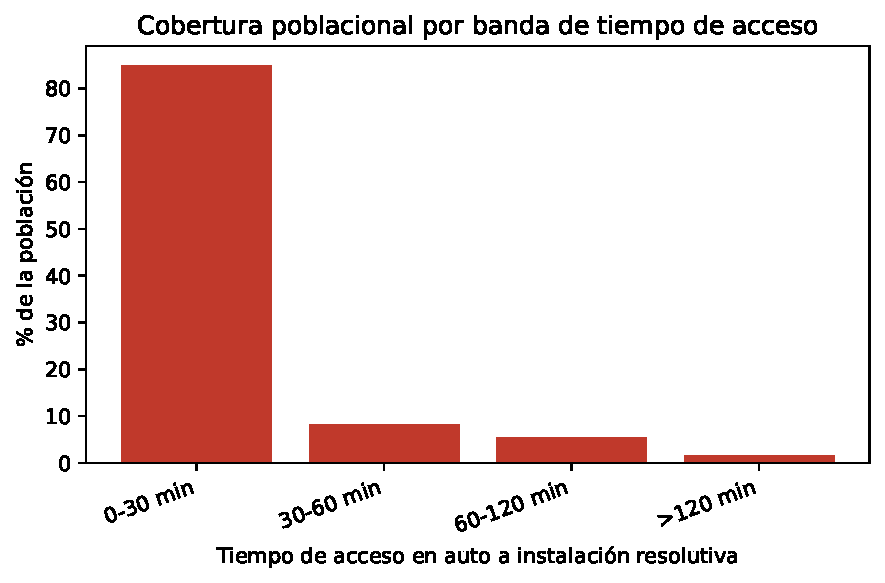
\includegraphics[width=0.75\textwidth]{figures/fig_coverage_bands.pdf}
\caption{Cobertura poblacional por banda de tiempo de acceso en auto,
Lambayeque.}
\end{figure}

\begin{figure}[h]
\centering
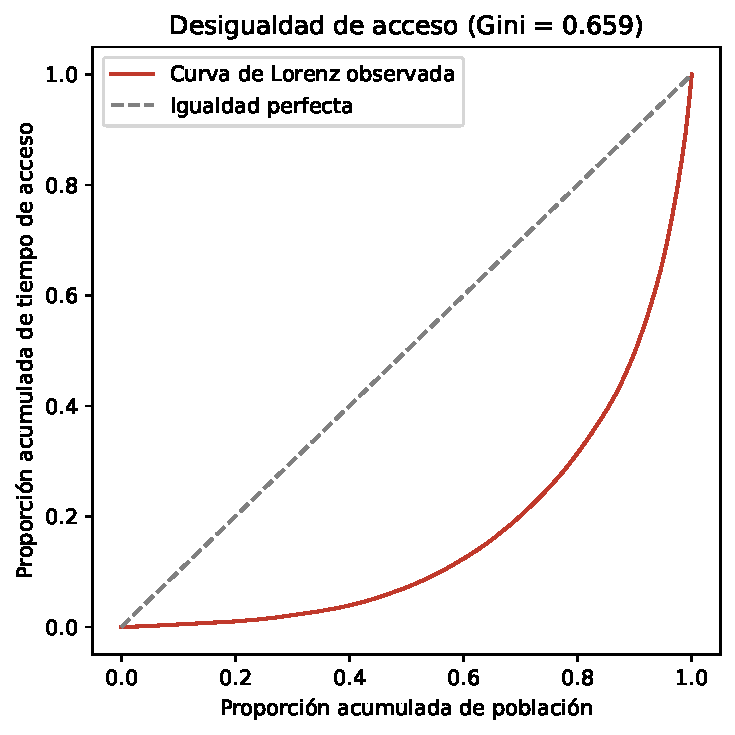
\includegraphics[width=0.6\textwidth]{figures/fig_lorenz_curve.pdf}
\caption{Curva de Lorenz del tiempo de acceso ponderado por población
(Gini = 0.659), Lambayeque.}
\end{figure}

\begin{figure}[h]
\centering
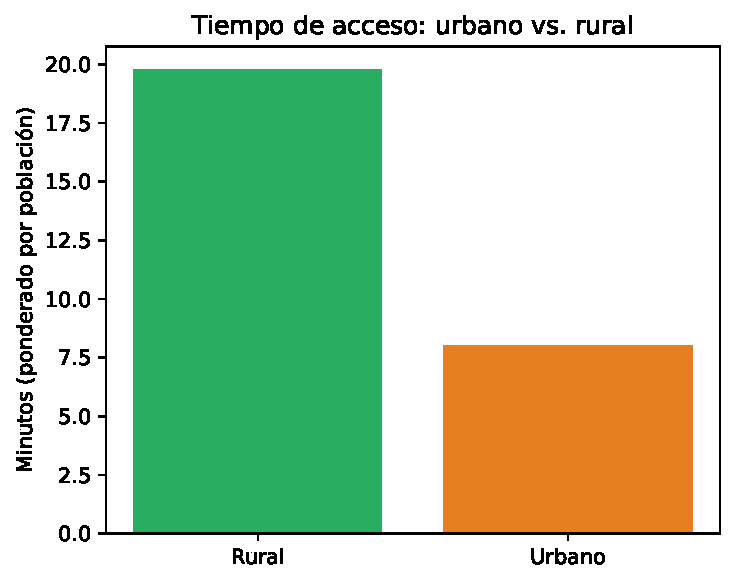
\includegraphics[width=0.6\textwidth]{figures/fig_urban_rural_contrast.pdf}
\caption{Tiempo de acceso ponderado: urbano (7.9 min) vs. rural (24.1 min),
Lambayeque.}
\end{figure}

\subsection{Brechas críticas}

\begin{table}[h]
\centering
\caption{Los 15 distritos con peor acceso ponderado por población}
\label{tab:critical-gaps}
\begin{tabular}{rrrrll}
\toprule
Acceso ponderado (min) & Población & Puntos de demanda & \% sin ruta & Departamento & Provincia \\
\midrule
182.15 & 7488.19 & 47.00 & 0.00 & LAMBAYEQUE & FERREÑAFE \\
152.97 & 7258.95 & 68.00 & 0.00 & LAMBAYEQUE & FERREÑAFE \\
99.98 & 37328.06 & 203.00 & 0.00 & LAMBAYEQUE & LAMBAYEQUE \\
93.74 & 5190.25 & 66.00 & 0.00 & LAMBAYEQUE & LAMBAYEQUE \\
85.25 & 5348.48 & 36.00 & 0.00 & LAMBAYEQUE & CHICLAYO \\
67.65 & 1755.71 & 6.00 & 0.00 & LAMBAYEQUE & CHICLAYO \\
67.31 & 791.44 & 9.00 & 0.00 & LAMBAYEQUE & LAMBAYEQUE \\
59.49 & 27021.28 & 87.00 & 0.00 & LAMBAYEQUE & LAMBAYEQUE \\
50.56 & 16914.21 & 61.00 & 0.00 & LAMBAYEQUE & CHICLAYO \\
43.71 & 14120.21 & 32.00 & 0.00 & LAMBAYEQUE & CHICLAYO \\
40.44 & 13572.04 & 62.00 & 0.00 & LAMBAYEQUE & LAMBAYEQUE \\
40.01 & 17030.87 & 82.00 & 0.00 & LAMBAYEQUE & FERREÑAFE \\
34.73 & 10606.83 & 33.00 & 0.00 & LAMBAYEQUE & CHICLAYO \\
30.90 & 8631.97 & 42.00 & 0.00 & LAMBAYEQUE & CHICLAYO \\
30.59 & 6525.75 & 27.00 & 0.00 & LAMBAYEQUE & CHICLAYO \\
\bottomrule
\end{tabular}
\end{table}


Los distritos de Cañaris y Ferreñafe (provincia de Ferreñafe, Lambayeque)
concentran el peor acceso ponderado, con más de 150 minutos promedio -- muy
por encima del umbral de 30 minutos que define la ``hora dorada''.

\section{Discusión: línea recta vs. red vial}

Para 1{,}833 puntos de demanda alcanzables en Lambayeque, la razón entre
distancia ruteada y distancia en línea recta (Haversine) al mismo destino
tiene mediana 1.17x y percentil 90 de 1.59x
(\texttt{data/outputs/straight\_line\_vs\_network.csv}). Es un desvío bajo,
consistente con el terreno predominantemente plano de la costa. La
expectativa -- a verificar cuando termine el ruteo de Cusco y Loreto -- es
que el factor de desvío sea sustancialmente mayor en Cusco por el relieve
andino (carreteras que serpentean valles y quebradas) y potencialmente
extremo o indefinido en Loreto, donde buena parte del territorio no tiene
red vial conectada y el transporte real ocurre por río -- un caso donde
ni la distancia en línea recta ni la ruteada por carretera reflejan el
verdadero costo de desplazamiento.

\section{Limitaciones}

\begin{itemize}
  \item \textbf{Cobertura de coordenadas}: 32.36\% de los establecimientos
  de RENIPRESS en los 3 departamentos (36.6\% a nivel nacional) no tienen
  coordenadas utilizables y quedan fuera del cómputo geoespacial -- el
  panorama real de oferta de salud es, en el peor caso, más denso de lo
  que este análisis puede ver.
  \item \textbf{Un establecimiento listado no implica uno operativo}:
  RENIPRESS es un registro administrativo; no confirma personal,
  equipamiento ni disponibilidad real en el momento de una emergencia.
  \item \textbf{Sin disponibilidad de ambulancias}: el análisis mide
  tiempo de viaje por red vial asumiendo un vehículo disponible de
  inmediato en el punto de demanda -- no incorpora tiempos de despacho,
  flota de ambulancias ni su ubicación real.
  \item \textbf{Población por punto es un supuesto, no una medición}: la
  ponderación por capital (departamental/provincial/distrital) que reparte
  la población censal 2017 entre centros poblados es una heurística
  documentada, no un dato observado. 6 distritos (Inkawasi, Villa Virgen,
  Villa Kintiarina y Megantoni en Cusco; Rosa Panduro y Yaguas en Loreto)
  fueron creados después del corte de la fuente de límites administrativos
  y quedan sin \texttt{ubigeo} de cruce.
  \item \textbf{Muestreo de puntos de demanda}: con 21{,}095 puntos de
  demanda frente a un tope de 5{,}000, se aplicó muestreo estratificado
  ponderado por población, lo que introduce error de muestreo respecto al
  universo completo, mayor cuanto más pequeño y disperso es el conjunto de
  un departamento.
  \item \textbf{Sesgo de cobertura de OpenStreetMap}: la completitud de la
  red vial de OSM es conocidamente desigual en zonas rurales y amazónicas
  de Perú; un desvío de ruteo alto o una desconexión de grafo en Loreto
  puede reflejar tanto la realidad geográfica como un vacío de mapeo.
  \item \textbf{Fragilidad de Overpass API}: la instancia por defecto de
  Overpass estuvo inalcanzable durante buena parte de la sesión de
  cómputo; aunque el pipeline hace \emph{failover} a espejos públicos, la
  dependencia de un servicio público compartido y no garantizado es en sí
  misma una limitación de reproducibilidad del pipeline en otra fecha.
  \item \textbf{Alcance de 3 departamentos}: los hallazgos no se
  extrapolan directamente a los 21 departamentos peruanos que quedan
  fuera del alcance.
\end{itemize}

\section{Conclusiones y recomendaciones}

Incluso en Lambayeque -- el departamento de mejor conectividad vial de los
tres en alcance -- el acceso a salud resolutiva es marcadamente desigual: un
Gini de 0.659 y una brecha de 3x entre acceso urbano y rural (7.9 vs.\
24.1 minutos) muestran que el promedio departamental esconde a los
distritos rurales de Ferreñafe, donde la ``hora dorada'' no existe en la
práctica (150+ minutos promedio ponderado). La recomendación de primer
orden, pendiente de confirmar con los resultados de Cusco y Loreto, es
priorizar la elevación de categoría de establecimientos I-3/I-4 ya
ubicados en esos distritos rurales -- exactamente el ejercicio que permite
el simulador de escenarios de la Fase 4 -- por sobre construir nueva
infraestructura desde cero.

\section{Referencias}

\begin{itemize}
  \item SUSALUD. Registro Nacional de Entidades Prestadoras de Servicios
  de Salud (RENIPRESS). \url{datosabiertos.gob.pe}. Consultado 2026-09-04.
  \item MINEDU. Sistema de Información Geográfica Educativa (SIGMED),
  Centros Poblados. \url{sigmed.minedu.gob.pe}. Consultado 2026-09-04.
  \item OpenStreetMap contributors. Perú extract. Geofabrik GmbH.
  \url{download.geofabrik.de}. Consultado 2026-09-04. Licencia ODbL.
  \item INEI. Censos Nacionales 2017: XII de Población, VII de Vivienda.
  Resultados Definitivos por departamento (Lambayeque, Cusco, Loreto),
  Tomo I. \url{inei.gob.pe}. Consultado 2026-09-04.
  \item Límites distritales derivados de cartografía INEI, republicados en
  \url{github.com/juaneladio/peru-geojson}.
  \item Boeing, G. (2017). OSMnx: New methods for acquiring, constructing,
  analyzing, and visualizing complex street networks. \emph{Computers,
  Environment and Urban Systems}.
\end{itemize}

\end{document}
